\documentclass{packages/labsec_planos}

%\usepackage[utf8]{inputenc}
%\usepackage[T1]{fontenc}
%\usepackage[brazil]{babel}
%\usepackage{longtable}
%\usepackage{colortbl}
%\usepackage[a4paper]{hyperref}
%\usepackage{indentfirst}
%\usepackage{cite}
% Para codigo fonte %
\usepackage{listings}
\lstset{
    literate={~} {$\sim$}{1}
}
%%%%%%%%% COLOCA MARCA D'AGUA DE RASCUNHO %%%%%%%%
%\usepackage{graphicx,type1cm,eso-pic,color}
%\makeatletter
%          \AddToShipoutPicture{
%            \setlength{\@tempdimb}{.5\paperwidth}
%            \setlength{\@tempdimc}{.5\paperheight}
%            \setlength{\unitlength}{1pt}
%            \put(\strip@pt\@tempdimb,\strip@pt\@tempdimc){
%        \makebox(0,0){\rotatebox{55}{\textcolor[gray]{0.85}
%        {\fontsize{5cm}{5cm}\selectfont{RASCUNHO}}}}
%            }
%        }
%\makeatother
%%%%%%%%% FIM DA MARCA D'AGUA DE RASCUNHO %%%%%%%%

\begin{document}

%%%%%%%%%%%%%%%%%%%
%% TUTILO E CAPA %%
%%%%%%%%%%%%%%%%%%%
\title{Manual do Desenvolvedor do SAEC}
\author{Pedro Henrique Lenzi Soares \\ Leandro Perin de Oliveira \\ João Victhor da Paz Campos \\ Vinícius Macelai}
%\dataDocumento{$ $Date$ $}
\dataDocumento{\today}
%\revisaoDocumento{$ $Revision$ $}
\logoLabsec{images-template/logoLabSEC.png}
%\logoLabsec{images-template/logoLabSEC.eps}
\logoINE{images-template/ine-ufsc.png}
%\logoINE{images-template/ine-ufsc.eps}
\nomeProjeto{Sistema Automatizado de Emissão de Certificados}

\maketitle

\clearpage

\tableofcontents

\chapter{Introdução}
TODO

\chapter{Instalação}
%%%%%%%%%%%%%%%%%%%%%
%% Instalação %%
%%%%%%%%%%%%%%%%%%%%%

\section{Introdução}
Esta seção tem como objetivo mostrar, passo a passo, como é feita a instalação e configuração do ambiente de desenvolvimento do SAEC. Deve-se levar em consideração que este documento foi produzido com base na instalação da versão 2.3 do SAEC, em um Ubuntu 14.04 de 64 bits.

%%%%%%%%%%%%%%%%%%%%%

\section{Repositório}
O código da aplicação encontra-se no GitLab do LabSEC e para acessá-lo é necessário possuir cadastro. É preciso também criar uma chave SSH e adicioná-la ao git, para que seja possível fazer o download do código da aplicação e realizar commits.

\subsection{Cadastro no GitLab LabSEC}
TODO

\subsection{Chave SSH}
O link abaixo deve ser utilizado para adicionar chaves SSH à sua conta do GitLab e verificar as que já foram adicionadas.

\begin{lstlisting}
    https://gitlab.labsec.ufsc.br/profile/keys
\end{lstlisting}

Para criar uma chave, o comando a seguir deve ser utilizado, com o seu email utilizado no GitLab.

\begin{lstlisting}[language=bash]
    $ ssh-keygen -t rsa -C "your.email@example.com" -b 4096
\end{lstlisting}

Recomenda-se utilizar o diretório padrão para salvar a chave (pressionando \textit{enter} quando o caminho for solicitado), e uma senha de sua escolha. Com a chave gerada, deve-se adicioná-la ao GitLab. Para imprimir a chave no terminal e copiá-la com \textit{Ctrl+Shift+C}, utilize o comando:

\begin{lstlisting}[language=bash]
    $ cat ~/.ssh/id_rsa.pub
\end{lstlisting}

\subsection{Download do Código}
Para baixar o código da aplicação e contribuir para o desenvolvimento da aplicação, é necessário fazer o download do \textit{git}.

\begin{lstlisting}[language=bash]
	$ sudo apt-get install git
\end{lstlisting}

No diretório de sua escolha, clone o repositório. Será criada uma pasta \textit{code}, que pode ser renomeada, com o código presente na branch \textit{master} do repositório.

\begin{lstlisting}[language=bash]
	$ git clone git@gitlab.labsec.ufsc.br:saec/code.git
\end{lstlisting}

Para fazer checkout do branch \textit{dev}, os seguintes comandos devem ser utilizados dentro da pasta onde o código está presente:

\begin{lstlisting}[language=bash]
	$ git fetch
	$ git checkout -b dev origin/dev
\end{lstlisting}

%%%%%%%%%%%%%%%%%%%%%

\section{Instalando Dependências}
Algumas dependências precisam ser instaladas para que seja possível utilizar o SAEC.

\begin{lstlisting}[language=bash]
	$ sudo apt-get install postgresql
	$ sudo apt-get install php5 php5-sqlite php5-ldap
	$ sudo apt-get install php5-mcrypt php5-dev php5-pgsql
	$ sudo apt-get install libapache2-mod-shib2
	$ sudo apt-get install libapache2-modsecurity
	$ sudo apt-get install libp11-dev
\end{lstlisting}

Deve-se, também, habilitar módulos do apache e do php.

\begin{lstlisting}
        $ sudo a2enmod ssl
        $ sudo a2enmod shib2
        $ sudo a2enmod rewrite
        $ sudo a2enmod headers
        $ sudo php5enmod mcrypt
\end{lstlisting}

TODO: ibcryptosec!

%%%%%%%%%%%%%%%%%%%%%

\section{Gerando Chave do Servidor HTTPS}

TODO

%%%%%%%%%%%%%%%%%%%%%

\section{Configurando o Banco de Dados}

TODO

%%%%%%%%%%%%%%%%%%%%%

\section{Apache Virtual Host}

TODO

%%%%%%%%%%%%%%%%%%%%%

\section{Testando Instalação}

TODO

\chapter{Libcryptosec}
TODO

\chapter{Configuração}
%%%%%%%%%%%%%%%%%%%%%
%% Configuração %%
%%%%%%%%%%%%%%%%%%%%%

\section{Introdução}
Antes de utilizar o SAEC de fato, é necessário passar por uma etapa de configuração do sistema. Acessando o sistema pela primeira vez com o endereço configurado no \textit{Virtual Host} do Apache, a página mostrada deve ser de login, assim como a figura \ref{fig:entrada}. Inicialmente, o usuário \textit{default} do sistema possui login "administrator" e senha "icpedu.

\begin{figure}[h]
     \centering
     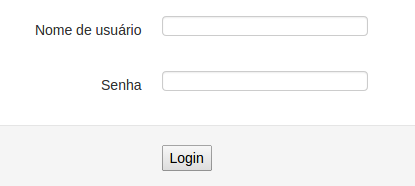
\includegraphics[scale=0.5]{images/entrada.png}
     \caption{Entrada no sistema}
     \label{fig:entrada}
\end{figure}

%%%%%%%%%%%%%%%%%%%%%

\section{Dados do Admin}
A primeira etapa do processo de configuração é a alteração do dados do administrador do sistema. Como trata-se de um ambiente de desenvolvimento, podemos utilizar dados falsos. Neste ponto, a "senha do usuário", que se refere à senha do usuário logado, ainda é a senha padrão, mas tenha em mente que a partir do momento que o formulário for submetido, o nome de usuário e senha escolhidos passarão a ser as novas credenciais do usuário administrador e serão exigidas nas próximas etapas de configuração. O usuário \textit{default} deixará de existir.

\begin{figure}[h]
     \centering
     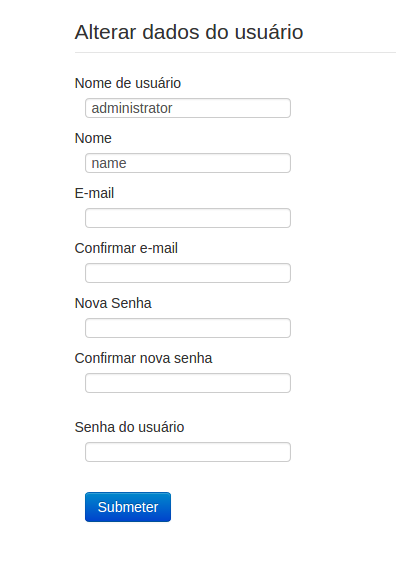
\includegraphics[scale=0.48]{images/inicioadmin.png}
     \caption{Dados do Admin}
     \label{fig:inicioadmin}
\end{figure}

%%%%%%%%%%%%%%%%%%%%%

\section{Restauração de Backup}
Em seguida, é dada a opção de inicializar o SAEC a partir de um backup previamente feito de outra instância da aplicação. É uma função muito útil em fase de testes de usuário, quando, por exemplo, for necessário limpar o banco de dados e reconfigurar o SAEC, ou quando a funcionalidade que deseja-se testar está incluída nos passos de configuração inicial do sistema. Caso seja recuperado algum backup, a aplicação é configurada automaticamente com as informações contidas nele, e a etapa de configuração é encerrada. Caso contrário, segue-se para o próximo passo.
    
    \begin{figure}[h]
     \centering
     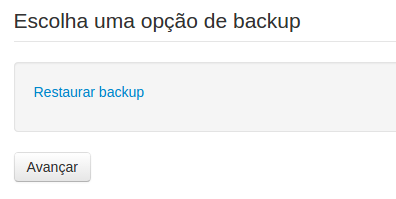
\includegraphics[scale=0.6]{images/opcaobackup.png}
     \caption{Restauração de Backup}
     \label{fig:opcaobackup}
\end{figure}

%%%%%%%%%%%%%%%%%%%%%

\section{Armazenamento de Chave}
Deve ser escolhido qual será o tipo de armazenamento utilizado para guardar a chave privada da Autoridade Certificadora do SAEC. Em ambientes de desenvolvimento, normalmente utilizamos "Chave em disco", embora seja necessário em alguns momentos, principalmente para testes, utilizar a opção "Módulo de Hardware Seguro", visto que em ambiente de produção é a opção que muito provavelmente deverá ser escolhida.
    
    \begin{figure}[h]
     \centering
     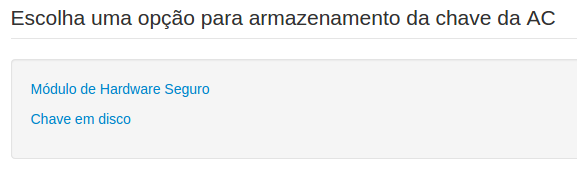
\includegraphics[scale=0.6]{images/armazenachave.png}
     \caption{Opção de armazenamento de chave}
     \label{fig:armazenachave}
\end{figure}

\subsection{Configuração do MSC}
Caso seja escolhida a opção que utiliza um Módulo de Segurança Criptográfico (MSC), é necessário salvar as configurações de acesso à ele, para que seja possível utilizar a chave privada da AC sempre que necessário.

TODO: explicar como se preenche esse form
    
    \begin{figure}[h]
     \centering
     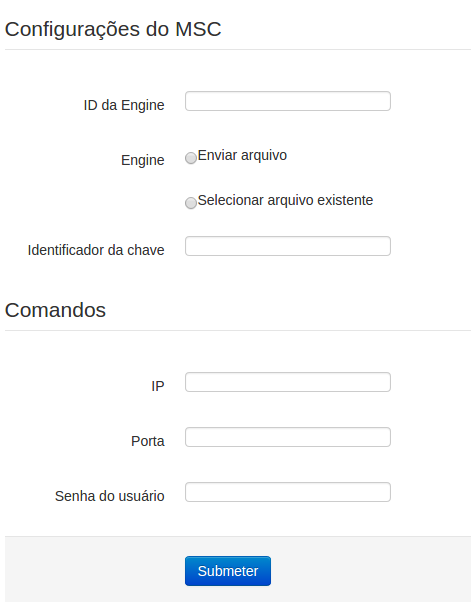
\includegraphics[scale=0.5]{images/confighsm.png}
     \caption{Configuração do MSC}
     \label{fig:confighsm}
\end{figure}

%%%%%%%%%%%%%%%%%%%%%

\section{Emissão do Certificado da AC}
\subsection{Criação da Requisição de Certificado}
TODO:refactor + printscreen

    Depois de configurá-lo, você será redirecionado para a página de criação de requisição para o seu sistema de emissão de certificados ICPEdu. Esta requisição deve ser aprovada por uma Autoridade Certificadora superior, que irá gerar um certificado para o sistema. 


\subsection{Emissão do Certificado}
TODO: guia para instalar SGCI na própria máquina e emitir certificado
    
    \begin{figure}[h]
     \centering
     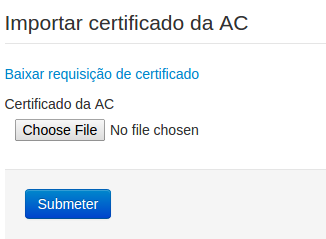
\includegraphics[scale=0.6]{images/importacertAC.png}
     \caption{Importação de certificado}
     \label{fig:reqcert}
\end{figure}


%%%%%%%%%%%%%%%%%%%%%

\section{Configuração de Certificado}
TODO: explain
    
    \begin{figure}[h]
     \centering
     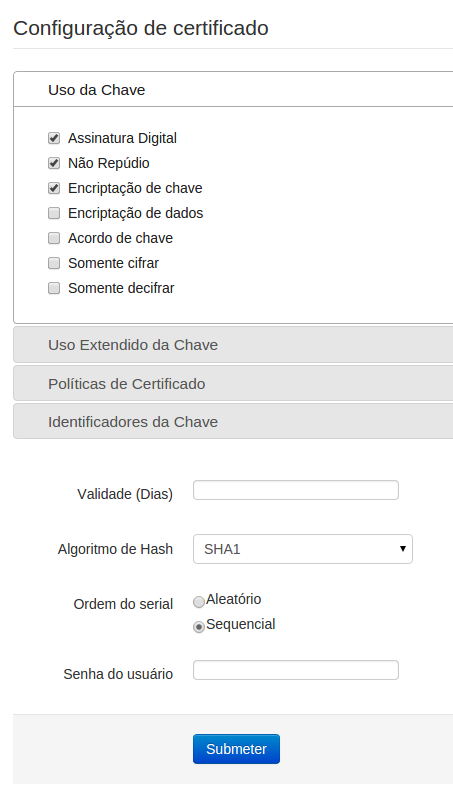
\includegraphics[scale=0.5]{images/configcertificado.png}
     \caption{Configuração do certificado}
     \label{fig:configcertificado}
\end{figure}

%%%%%%%%%%%%%%%%%%%%%

\section{Whitelist}
TODO: explain + printscreen

%%%%%%%%%%%%%%%%%%%%%

\section{Federação}
TODO:explain
    
    ... é selecionar a federação a qual o seu sistema pertence. É possível selecionar a Comunidade Acadêmica Federada (CAFe) ou a Chimarrão. Pode-se ainda escolher outra federação não listada, e neste caso deve-se fornecer as URLs da mesma.
    
%%%%%%%%%%%%%%%%%%%%%
    
\section{Registro de Operador}
TODO:explain
    
    \begin{figure}[h]
     \centering
     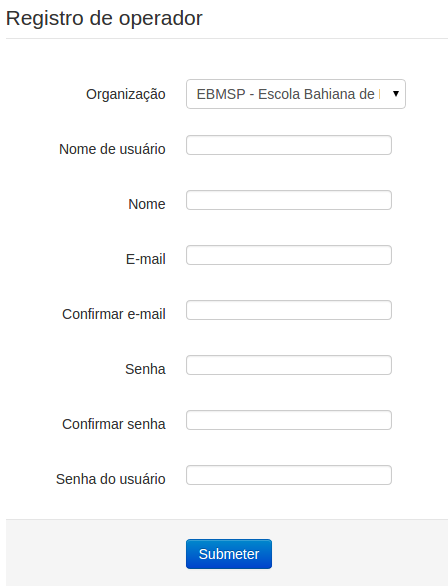
\includegraphics[scale=0.5]{images/inicioregistroop.png}
     \caption{Registro de operador}
     \label{fig:inicioregop}
\end{figure}

TODO:decidir sobre deixar ou não figura da página inicial...
    
    \begin{figure}[h]
     \centering
     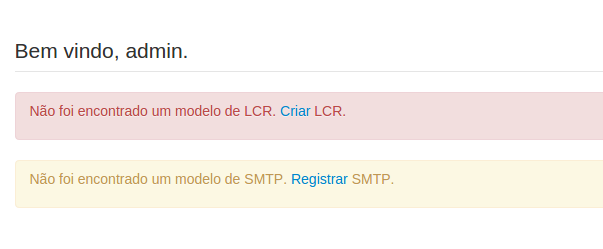
\includegraphics[scale=0.5]{images/pendencias.png}
     \caption{Tarefas pendentes}
     \label{fig:pendencias}
\end{figure}

\chapter{Desenvolvimento}
%%%%%%%%%%%%%%%%%%%%%
%% Desenvolvimento %%
%%%%%%%%%%%%%%%%%%%%%

\section{Introdução}

A partir deste ponto, o ambiente de trabalho está pronto para ser utilizado. Neste capítulo, são apresentados detalhes do processo de desenvolvimento, e nos próximos, detalhes sobre funcionalidades específicas do sistema e fragmentos de código, tornando facilmente adquirível o conhecimento necessário para fazer alterações, aprimoramentos e correções na aplicação. 

%%%%%%%%%%%%%%%%%%%%%

\section{Repositório}

\subsection{Organização do Repositório}
O SAEC é dividido em 4 repositórios diferentes:
    \begin{itemize}
        \item \textbf{code}: código da aplicação;
        \item \textbf{phplibcryptosec}: código do wrapper PHP5LibCryptoSec;
        \item \textbf{makepkg}: script para a geração do pacote de instalação da aplicação;
        \item \textbf{doc}: documentação do projeto.
    \end{itemize}

\vspace{5mm}

O repositório principal, \textit{code}, está dividido em diversas branches:
    \begin{itemize}
        \item \textbf{master}: é atualizado quando uma nova versão é lançada;
        \item \textbf{dev}: é o mais utilizado durante o desenvolvimento;
        \item \textbf{release}: utilizado para maturação de uma nova versão;
        \item \textbf{SAEC-X}: utilizados para a realização de tarefas.
    \end{itemize}

\begin{figure}[h]
  \begin{center}
    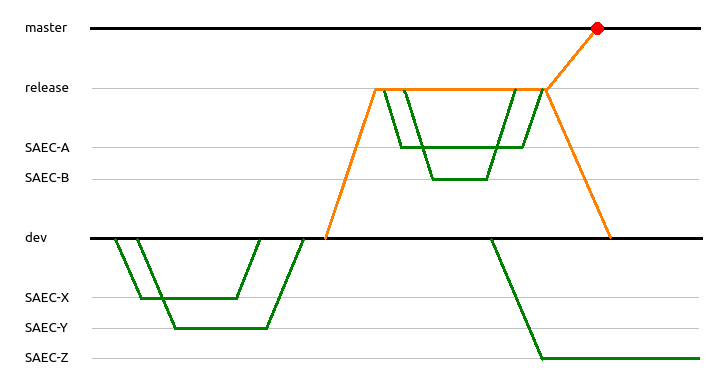
\includegraphics[scale=0.58]{images/git.png}
    \caption{Fluxo do Repositório}
    \label{fig:fluxobranches}
  \end{center}
\end{figure}

\vspace{5mm}

O fluxo do repositório, representado pela figura \ref{fig:fluxobranches}, funciona da seguinte maneira: Para cada tarefa de desenvolvimento é criado um novo branch temporário com o nome \textbf{SAEC-X}, onde X é um número que identifica a tarefa. Quando a tarefa é concluída, deve ser aberto um \textit{merge request} para o branch \textbf{dev}. Quando julgar-se necessário o lançamento de uma nova versão do software com as alterações contidas no \textbf{dev}, é feito um \textit{merge} dele para o branch \textbf{release} e é lançada uma nova versão para testes, com o código contido neste branch. Após realizados os testes e as correções necessárias, são feitos \textit{merges} do branch \textbf{release} para o \textbf{dev} (para incluir nele as correções feitas) e \textbf{master}, onde é criada uma \textit{tag} para a nova versão.

\subsection{Usando o Git}

Para começar o desenvolvimento de uma tarefa, deve-se primeiro verificar se o branch local é o \textit{dev}. Para isso, no diretório onde está o código, o comando \textit{branch} pode ser executado. Caso não seja, basta realizar um \textit{checkout}.

\begin{lstlisting}[language=bash]
    $ git branch
    $ git checkout dev
\end{lstlisting}

Estando no branch \textit{dev}, deve-se realizar um \textit{pull} do repositório para atualizar o código local e criar um novo branch \textit{SAEC-X}, onde X é o número que identifica a tarefa que será realizada.

\begin{lstlisting}[language=bash]
    $ git pull origin dev
    $ git checkout -b SAEC-X
\end{lstlisting}

Terminado o desenvolvimento, podem ser utilizados os comandos \textit{status} e \textit{diff} para visualizar as alterações feitas. Caso seja necessário reverter as alterações em algum arquivo, basta utilizar o comando:

\begin{lstlisting}[language=bash]
    $ git checkout -- <caminho_do_arquivo>
\end{lstlisting}

Após verificar que as alterações feitas estão corretas, pode ser feito o commit.

\begin{lstlisting}[language=bash]
    $ git add -A
    $ git commit -m "SAEC-X: Mensagem descrevendo o que foi feito"
    $ git push origin SAEC-X
\end{lstlisting}

Feito o commit, deve-se então entrar no GitLab e criar um \textit{merge request}, para que seu código seja revisado e incluído na branch \textit{dev}.

\chapter{Tipos de Usuários}
%%%%%%%%%%%%%%%%%%%%%
%% Tipos de Usuários %%
%%%%%%%%%%%%%%%%%%%%%

\section{Introdução}
O SAEC possui 4 diferentes tipos de usuários, cada qual com suas funções e permissões.

%%%%%%%%%%%%%%%%%%%%%

\section{God}
No SAEC não existe uma categoria diferente de usuário para o usuário \textbf{criador}, e ele é visto como um \textit{administrator} perante o sistema. No entando, consideramos que durante o processo de configuração do SAEC, o primeiro \textit{admin}, que executa o processo, é o criador.

Este conceito é importante, pois o usuário \textit{administrator} não pode ter acesso às páginas da etapa de configuração do sistema após encerrada essa etapa.

%%%%%%%%%%%%%%%%%%%%%

\section{Administrator}
TODO

%%%%%%%%%%%%%%%%%%%%%

\section{Operator}
O usuário \textbf{operador} está fortemente relacionado à uma instituição. Ele é responsável por garantir que a relação entre o SAEC e a instituição que representa esteja correta.

%%%%%%%%%%%%%%%%%%%%%

\section{Default}
O usuário \textbf{default}, ou usuário comum, é aquele que não está \textit{logado}. Trata-se dos clientes do serviço, que o acessam para a emissão de certificados.

\chapter{Estrutura de Arquivos}
%%%%%%%%%%%%%%%%%%%%%
%% Estrutura de Arquivos %%
%%%%%%%%%%%%%%%%%%%%%

\section{Introdução}
Neste capítulo, é explicado como os arquivos do projeto são separados e organizados. É importante saber que para o desenvolvimento do SAEC utilizamos um Framework para PHP chamado Zend Framework, o que influenciou em algumas decisões quanto à estrutura dos arquivos.

%%%%%%%%%%%%%%%%%%%%%

\section{./application}
No diretório \textit{./application} está contida a maior parte do projeto, que são os \textit{modules}, juntamente com alguns outros arquivos.

\subsection{Modules}
Existem 7 \textit{modules}:
    \begin{itemize}
        \item admin
        \item oper
        \item default
        \item common
        \item db
        \item cron
        \item auth
    \end{itemize}

Nos \textit{modules} \textbf{admin}, \textbf{oper} e \textbf{default} estão as funcionalidades exclusivas de cada tipo de usuário, administrador, operador e usuário comum, respectivamente. Em \textbf{common}, estão funcionalidades que são comuns à mais de um tipo de usuário. Em cada um desses quatro, existem \textit{Controllers}, \textit{Forms} e \textit{Views}, que serão explicados no final deste capítulo.

No \textit{module} \textbf{db}, encontram-se os arquivos referentes ao banco de dados. Tanto scripts de criação e deleção do banco de dados, como \textit{DbTables} e \textit{Mappers}. Em \textbf{cron}, estão funcionalidades que podem ser executadas automaticamente pelo \textit{cron}. O \textbf{auth} é exclusivo para as ferramentas de autenticação de usuário.

\subsection{Configs}
Dentro deste diretório, existem apenas 2 arquivos. No \textit{local.ini} estão as configurações locais para o banco de dados, e no \textit{application.ini} algumas outras configurações do projeto.

\subsection{Languages}
Em \textit{languages}, estão os arquivos de traduções. Existe um arquivo \textit{.mo} ilegível para cada idioma suportado pelo sistema, que é gerado automaticamente a partir do arquivo \textit{.po} do idioma. O arquivo \textit{.po}, que é o que pode ser editado para que a tradução de uma nova frase seja incluída no sistema, contém mensagens no seguinte formato:

\begin{lstlisting}
    msgid "hello_world"
    msgstr "Hello, world!"
\end{lstlisting}

Em \textit{msgid} fica um identificador para cada mensagem, e em \textit{msgstr} a mensagem no idioma escolhido. Por convenção, no SAEC utilizamos como id da mensagem a própria mensagem, em inglês. Para gerar os novos arquivos \textit{.mo} após modificar os \textit{.po}, o script \textit{convertpten.sh} deve ser executado.

\subsection{Layouts}
Em \textit{layouts} encontra-se um arquivo \textit{.phtml} que define o \textit{layout} comum à todas as páginas da aplicação e um arquivo \textit{.xml} que contém os links dos dropdowns da barra de menus do sistema.

%%%%%%%%%%%%%%%%%%%%%

\section{./library}
Neste diretório encontram-se bibliotecas utilizadas no projeto. Existem arquivos do Zend Framework e do PHP5LibcryptoSec, além de alguns que foram separados para formar uma biblioteca própria do SAEC.

%%%%%%%%%%%%%%%%%%%%%

\section{./public}
TODO

%%%%%%%%%%%%%%%%%%%%%

\section{./scripts}
TODO

%%%%%%%%%%%%%%%%%%%%%

\section{./tests}
TODO

%%%%%%%%%%%%%%%%%%%%%

\section{Fluxo de Execução de uma Funcionalidade}
Para entender como funciona o fluxo de execução, podemos exemplificar com uma simples funcionalidade que acesse o banco de dados, como por exemplo, criar um usuário.

\subsection{Componentes Principais}

Cada funcionalidade deste tipo possui diversos componentes:
    \begin{itemize}
        \item Controller
        \item Form
        \item View
        \item DbTable
        \item Mapper
        \item Model
    \end{itemize}

Podemos considerar o \textbf{controller} como o principal componente da estrutura. Levando em conta nosso exemplo, encontraríamos nele algum método com o nome \textit{createuserAction}. Neste método instanciamos o \textbf{form}, que contém o formulário que deve ser apresentado ao usuário quando este acessar a página de criar um usuário. A \textbf{view} estará automaticamente ligada com o \textbf{controller} se o nome do arquivo for \textit{createuser.phtml}, por causa do \textit{Zend Framework}. Ela possui o \textit{HTML}, \textit{CSS}, \textit{JavaScript} e até mesmo alguns trechos em \textit{PHP} que formam a página \textit{web} que será mostrada ao usuário. Para que a \textbf{view} possa utilizar o \textbf{form}, no \textbf{controller} escrevemos a seguinte linha de código:

\begin{lstlisting}[language=php]
    $this->view->viewForm = $controllerForm
\end{lstlisting}

Onde \textit{\$controllerForm} é a instância criada, e \textit{viewForm} é a variável da \textbf{view} que armazenará a instância do \textbf{form}.

A \textbf{DbTable} é basicamente um arquivo que define como é a tabela presente no banco de dados, contendo informações sobre as colunas e chaves da tabela. Ela é utilizada pelo \textbf{Mapper}, que contém métodos para executar consultas no banco de dados. Muitos deles utilizam funções prontas que o \textit{Zend Framework} disponibiliza, outros possuem \textit{queries} \textit{SQL}. Para que objetos que representam linhas do BD sejam transportados entre o \textbf{mapper} e \textbf{controller} de uma forma mais organizada, existe o \textbf{model}, que é uma classe simples, com atributos que representam cada coluna da tabela no BD e \textit{getters} e \textit{setters}.

Quando o formulário é submetido pelo usuário, o \textbf{controller} analisa as informações enviadas e faz as alterações necessárias no BD utilizando os métodos disponibilizados pelo \textbf{mapper}.

Cada action pode ser acessada no navegador através do link \textit{link/module/controller/action}, como por exemplo \textit{https://localhost:40444/admin/user/createuser} para a action \textit{createuserAction}, do controller \textit{userController}, do module \textit{admin}.

\subsection{Arquivos Importantes}

Além deles, não se pode esquecer de alguns arquivos que também possuem informações sobre cada funcionalidade:
    \begin{itemize}
        \item Script de criação do BD
        \item navigation.xml 
        \item Acl
    \end{itemize}

No script de criação do BD (\textit{./application/modules/db/sql/createDatabase.sql}) estará o \textit{SQL} responsável por criar cada tabela, e deve ser consultado/alterado quando necessário.

Em \textit{./application/layouts/scripts/navigation.xml} estão os links dos menus, e deve ser alterado para adicionar links para as novas funcionalidades.

Já a \textbf{Acl} (\textit{./library/SAEC/Acl.php}) é quem controla qual tipo de usuário tem acesso a cada página. Ela deve ser sempre alterada quando uma nova funcionalidade é criada, para que o usuário à quem ela for destinada tenha permissão de acesso.





\chapter{Mapeador de Atributos}
TODO

\chapter{Shibboleth}
%%%%%%%%%%%%%%%%%%%%%
%% Desenvolvimento %%
%%%%%%%%%%%%%%%%%%%%%

\section{Introdução}

Para algumas funcionalidades do SAEC, inclusive a emissão de certificados, é utilizado o Shibboleth para autenticação perante alguma universidade. Quando um usuário solicita alguma dessas funcionalidades, ele é redirecionado para o serviço de WAYF (Where Are You From) para informar qual a sua instituição. Após isso, é redirecionado para uma página de autenticação da sua instituição, que chamamos de IDP (Identity Provider). Feita a autenticação, ele é redirecionado novamente para o SAEC, e os dados da autenticação são salvos em variáveis de sessão.

%%%%%%%%%%%%%%%%%%%%%

\section{Funcionalidades Envolvidas}

As funcionalidades que necessitam autenticação perante instituição podem ser divididas em dois grupos, diferenciando-as quanto à utilização ou não utilização do mapeador de atributos.

As que o utilizam para mapear os dados vindos da IDP são:
\begin{itemize}
    \item Emissão de Certificado
    \item Revogação de Certificado
    \item Instalação de Certificado
    \item Validação de Atributos
\end{itemize}

As que não o utilizam são:
\begin{itemize}
        \item Configuração do Mapeador de Atributos
        \item Pedido de Operador
\end{itemize}

Após realizada a autenticação perante instituição, o usuário é redirecionado de acordo com o arquivo ./public/signup/index.php. Se a funcionalidade requerida for uma que não utiliza o mapeador de atributos, ele é redirecionado diretamente para a página, se não, para o \textit{SignUpController}, onde os atributos são mapeados de acordo com a configuração salva no banco de dados, e somente após isso acontece o redirecionamento para a página requerida.

\chapter{SMTP}
TODO

\chapter{Cron}
TODO

\chapter{Deploy}
TODO

\end{document}
